\documentclass[../../main.tex]{subfiles}
\begin{document}

\subsection*{2.7}
Due piani indefiniti paralleli, distanti $d = 20\ cm$, sono carichi ocn densità uniformi $\sigma_1=17.72 * 10^{-8}\ \frac{C}{m^2}$ e $\sigma_2 = \frac{\sigma_1}{2}$
\\a) Determinare il potenziale V(x), ponendonolo uguale a 0 nel punto di mezzo O tra i due piani.
\\b) Determinare l'energia cinetica minima $E_{k_{min}}$ che deve avere un protone nel punto A(x = -d) per giungere in un generico punto O'. Se un elettrone viene lasciato libero in A con v=0 dove arriva?
\\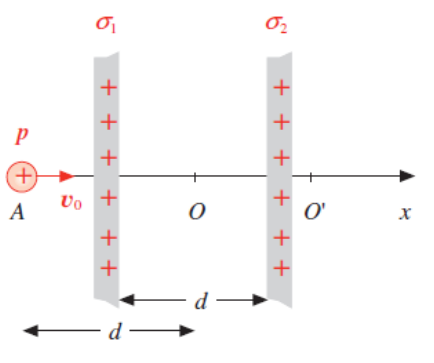
\includegraphics[scale=0.3]{e_2_7_0.png}
\\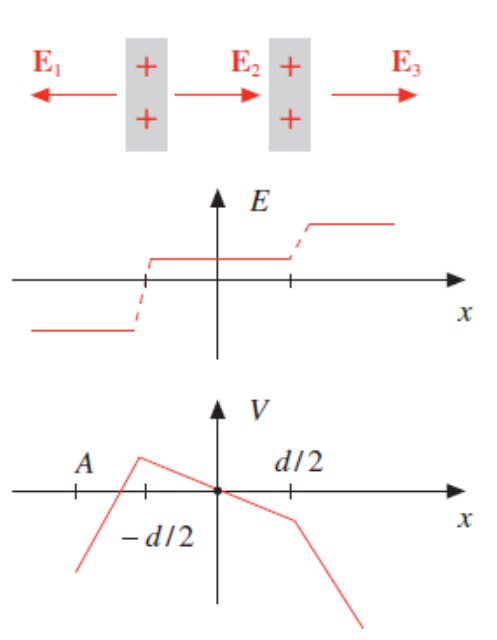
\includegraphics[scale=0.3]{e_2_7_1.png}
\subsubsection*{Formule utilizzate}
\subsubsection*{Soluzione punto a}
per: $x < -\frac{d}{2}$:
\\$E_1 = -\frac{\sigma_2 + \sigma_1}{2\epsilon_0}\vec{u_x} = \frac{3\sigma_2}{2\epsilon_0}\vec{u_x} = 1.5 * 10^4\vec{u_x}\ \frac{V}{m}$
\\$\sigma_1 = 2\sigma_2$
\\$V_1(x) = \frac{\sigma_2}{2\epsilon_0}(3x + 2d)$
\\per $-\frac{d}{2} < x < \frac{d}{2}$:
\\$E_2 = \frac{\sigma_1 - \sigma_2}{2\epsilon_0}\vec{u_x} = \frac{\sigma_2}{2\epsilon_0}\vec{u_x} = 0.5*10^4\vec{u_x}\ \frac{V}{m}$
\\$\sigma_1 = 2\sigma_2$
\\$V_2(x) = -\frac{\sigma_2}{2\epsilon_0}x$
\\per $x > \frac{d}{2}$
\\$E_3 = \frac{\sigma_1 + \sigma_2}{2\epsilon_0}\vec{u_x} = 1.5 * 10^4 \vec{u_x}\ \frac{V}{m}$
\\$V_3(x) = \frac{\sigma_2}{2\epsilon_0}(-3x+d)$
\\Per raggiungere la regione $x > \frac{d}{2}$ il protone deve attraversare le barriere del potenziale, cioè deve salire fino al punto di potenziale maggiore a $x = -\frac{d}{2}$. Una volta raggiunto quel punto, verrà spinto completamente a destra. Pertanto l'energia cinetica iniziale deve essere almeno uguale alla differenza di potenziale.
\\$\Delta v=v_i(-\frac{d}{2})-V_1(A) = \frac{3\sigma_2 d}{4\epsilon_0} = 1500V $
\\$E_{k_{min}} = 1.5 keV$
\\L'elettrone viene accellerato verso dx fino a $x = -\frac{d}{2}$ quindi viene decelleratore.
\\Usando la conservazione dell'energia, l'elettrone si ferma nel punto dell'asse x posto tale che $V(x) = V(a)$.
\\$\frac{\sigma_2}{2\epsilon_0}(-3x+d) = - \frac{\sigma_2}{2\epsilon_0}d$ per cui $x = \frac{2d}{3} = 13.3\ cm$


\subsubsection*{Soluzione punto b}
\newpage

\end{document}